\hthree{MariaDB vs. MySQL}

\begin{figure}[H]
    \centering
    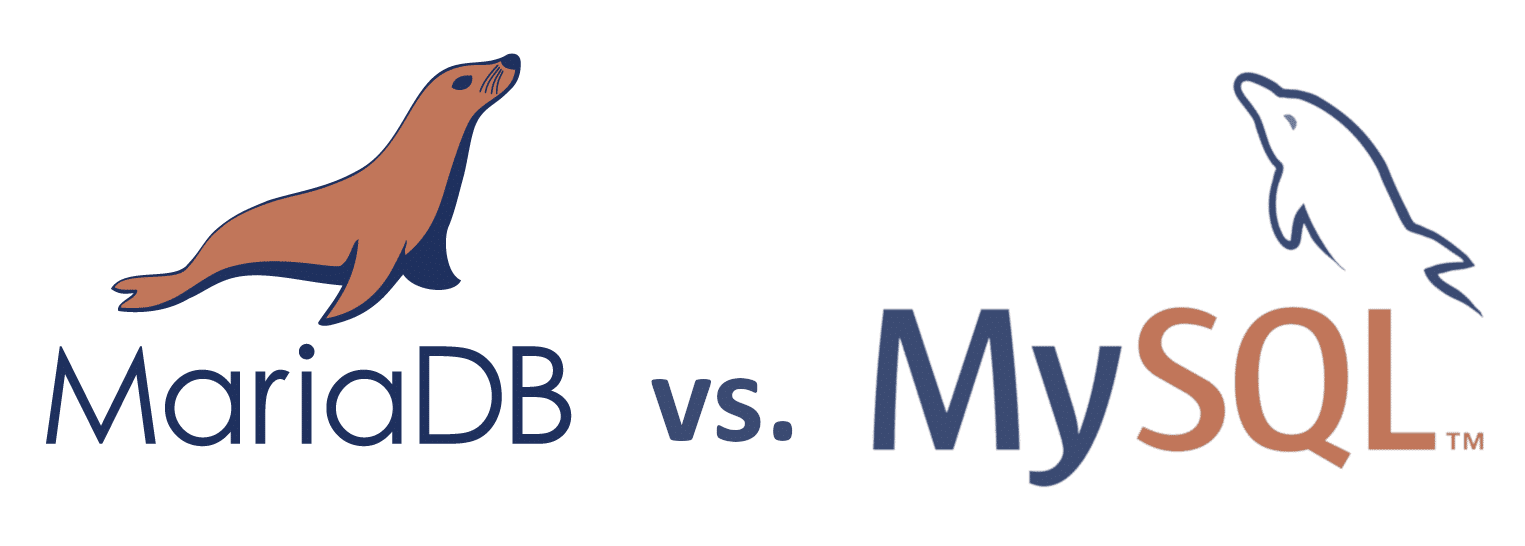
\includegraphics[width=\textwidth]{media/MariaDB/mariavsmy.png}
    \caption{MariaDB vs. MySQL \cite{MariaVsMyBild}}
    \label{fig:MariavsMy}
\end{figure}

2009, als MariaDB ins Leben gerufen wurde, konnte MySQL schon auf Erfahrung und Wissen aus 20 Jahren zurückgreifen. Zu Beginn des neuen Datenbanksystems, waren die Unterschiede der beiden noch gar nicht so groß und MariaDB wollte den primären Fokus auf einen smarten Support von Systemen und das Abwickeln sauberer Weiterentwicklung legen, welche durch die Open-Source Community getragen werden. Mittlerweile verfolgen beide Unternehmen und Datenbankmanagementsysteme konträre Produktionsansätze und Zugänge zu Problemlösungen im Datenverwaltungsbereich in den 20ern der 21. Jahrhundert. \cite{MariaVsMy}

MySQL und MariaDB basieren beiden auf dem gleichen Softwarekern. MariaDB wurde damals als Abspaltung (Fork) von der MySQL Version 5.1 ins Leben gerufen und entwickelte im Laufe der Zeit immer mehr an Selbstständigkeit und Unabhängigkeit zu MySQL. Im nachfolgenden Vergleich wird auf die Unterschiede zwischen MySQL MariaDB eingegangen. \cite{MariaVsMy}

\hfour{Datenbankstruktur}

Eines der Ziele, welche sich MariaDB zu Beginn gesetzt hat, war eine Gesamtkompatibilität zwischen den beiden Datenbankmanagementsystemen herzustellen. Das heißt, dass ein Wechsel zwischen MySQL und MariaDB oder umgekehrt, aber auch ein Umstieg zwischen unterschiedlichen MySQL Versionen problemlos funktionieren soll. Dieses Kriterium wurde von Seiten MariaDB bis zur MySQL Version 7 umgesetzt. \cite{MariaVsMy}

Im Prinzip kann aber gesagt werden, dass beide Datenbanksysteme die gleiche Datenstruktur verwenden, da die beide zur Gattung der relationalen Datenbanksysteme gehören. Deshalb gibt es in vielen Bereichen eine schon oben erwähnte Kompatibilität zum Beispiel im Bereich der Daten- und Tabellendefinition, aber auch im Gebiet von Protokollen, Strukturen oder Entwicklungsschnittstellen. Weiters wurden auch einige Befehle für Administrationsaufgaben oder das Erstellen von Backups übernommen. Hier kann man auf "mysqldump" oder "mysqladmin" hinweisen. \cite{MariaVsMy}

Die Kompatibilität wurde von MariaDB immer sehr großgeschrieben. Deshalb wurde der Code einmal im Monat mit jenem von MySQL abgeglichen. Dieser Einklang wurde mit dem Herausgeben von MySQL Version 8 jedoch beendet. Seither gilt diese Binärkompatibilität als beendet und man kann nicht mehr problemlos zwischen MySQL und MariaDB wechseln. Weiters ist MySQL auch seit Version 8.0 auch innerhalb des Systems nicht mehr abwärtskompatibel. \cite{MariaVsMy}

Eines der Beispiele, dass sich MySQL und MariaDB in der zukünftigen Entwicklung voneinander wegbewegen und unterschiedliche Weg einschlagen werden ist das Implementieren des sogenannten "Data-Dictionary" welches transaktional arbeitet und seit MySQL Version 8 enthalten ist. Dieses Konzept unterscheidet sich in Grundlegenden Punkten von vorhergegangenen Versionen. Dieses Konzept ist zur  Verarbeitung von Metadaten eingebaut worden. Da MariaDB zurzeit nicht wissentlich an einem vergleichbaren Mechanismus arbeitet ist davon auszugehen, dass in Zukunft auch keine Kompatibilität im Bereich von Datafiles geben wird. \cite{MariaVsMy}

\hfour{Datenbank-Engines}

Eine Datenbank-Engine ist ein sogenanntes Speichersubsystem, welches für das Erstellen, Lesen, Manipulieren und Löschen von Daten zuständig ist. Ohne diese Engine wäre dies für das Datenbankmanagementsystem nicht möglich.
MariaDB möchte sich in diesem Bereich durch eine stetig wachsende Anzahl an unterstützen Engines von MySQL unterscheiden. Dies hat den Vorteil, dass man bei der Auswahl eine höhere Flexibilität genießt. \cite{MariaVsMy}

Als Beispiel für eine von beiden Seiten kompatible Engine kann man InnoDB nennen. InnoDB kommt seit MySQL Version 5.5 und seit MariaDB Version 10.2 als Standardengine zum Einsatz und bietet bei beiden Datenbanksystemen einen transaktionssicheren Lese- und Schreibzugriff. \cite{MariaVsMy}

MariaDB unterstützt jedoch mit 19 Datenbank-Engines eine deutlich höhere Anzahl als MySQL, welche nur acht unterstützen. Als Beispiel für eine nur von MariaDB angebotene Engine kann man TukoDB nennen, welche auf die Verarbeitung von großen Datenmengen spezialisiert ist und damit perfekt für den "Big Data" Anwendungsbereich optimiert ist. \cite{MariaVsMy}

\hfour{Datenbankabfrage}

In diesem Punkt gibt es keinerlei Unterschiede zwischen den Systemen. \cite{MariaVsMy}

\hfour{Performance}

Das Liefern von Leistung wird in vielen Unternehmen der ausschlaggebendste Punkt in Bezug auf die Wahl des Datenbanksystems sein. Sollte sich eine Firma nun für ein von Michael Widenius entworfenes Produkt (MySQL oder MariaDB) entscheiden, stellt sich die Frage, welches der beiden Datenbankmanagementsystemen schafft es dem Unternehmen eine höhere Performance zu liefern. Wenn auf die blanken Ergebnisse eines Benchmark-Tests (wie des DBT-3) geblickt wird hat MariaDB die Nase vorne, jedoch macht hierbei vor Allem die verwendete Datenbank-Engine den Unterschied. \cite{MariaVsMy}

Es kann jedoch gesagt werden, dass sehr viel von dem Entwickler abhängt, da es immer darauf ankommt, was für welchen Anwendungsfall verwendet und implementiert wird. Hierbei kommt es wie schon oben erwähnt auf die verwendete Datenbank-Engine an. In diesem Punkt kann MariaDB besonders punkten, da es viele alternative Engines unterstützt. MariaDB liefert seit Version 10.0.1 seinen Kunden eine zusätzliche Optimierung der SQL-Abfragen, da nun nicht mehr auf interne Statistiken der Datenbank-Engine vertraut wird, sondern diese innerhalb des Systems berechnet und als normale Tabelle abgespeichert werden. So kann man schneller und engineunabhängig den besten Weg für SQL-Kommandos ermitteln. \cite{MariaVsMy}

\hfour{Hochverfügbarkeit}

Beide Systeme können Technologien liefern, welche für den Hochverfügbarkeitsbereich eingesetzt werden können.

MySQL verwendet eine Datenbankkonstruktion (Clustertechnologie), welche transaktionssicher, in Echtzeit und nach den Prinzipien von ACID (Atomicity, Consistency, Isolation, Durability) arbeitet. Durch die Verteilung des gesamten Systems kann man es verhindern, dass sich im Clustersystem ein "Single Point of Failure" ergibt und man so eine Verfügbarkeit von 99,9999\% erreicht. Der Zugriff kann dann je nach Bedarf entweder per SQL oder NoSQL erfolgen. Außerdem wird das gesamte Clusterservice von MySQL immer als selbstständiges Release angeboten (aktuelle Version 7.5) \cite{MariaVsMy}

Bei MariaDB sieht das Ganze ein bisschen anders aus, da sie im Bereich von Cluster auf die externe Clustertechnologie "Galera" setzten. Die Verbindungsstelle dazu wurde seit MariaDB Version 10.1 standardmäßig implementiert. Der Nachteil hierbei ist jedoch, dass die einzig unterstützte Datenbank-Engine bei Verwenden von "Galera" (Clusterbetrieb) nur InnoDB ist. \cite{MariaVsMy}

\hfour{Sicherheit}

Im Bereich der Sicherheit setzten beide Datenbanksysteme auf das Verschlüsseln von Daten, das Authentifizieren und das Hinzufügen von unterschiedlichen Benutzern mit unterschiedlichen Rechten. \cite{MariaVsMy}

MySQL setzt hierbei auf eine Verschlüsselung, welche mithilfe der Standarddatenbank-Engin (InnoDB) vollzogen wird. Der große Nachteil hierbei ist, dass das Verschlüsseln einzelner Tabellen nicht möglich ist und immer nur auf den gesamten Tablespace (logische Speichereinheit in InnoDB, welche die Gesamtheit der Daten umfasst) angewandt werden kann. \cite{MariaVsMy}

MariaDB geht seit Version 10.1 einen anderen Weg, welcher deutliche Verbesserungen im Bereich der Verschlüsselung mit sich bringt. Konkret bedeutet das, dass so eine Verschlüsselung auf unterschiedlichen Ebenen der Datenbank möglich ist. Wenn man einige Beispiele für dieses Ebenen nennen möchte, dann kann man dies durch InnoDB-Tabellenräume, Aria Tabellen oder Binäre Logdaten. \cite{MariaVsMy}

Weiters implementierte MariaDB sogenannte "Rolling Encryption Keys", welche eine Verschlüsselung mit Ablaufdatum ermöglichen und so keine dauerhafte Verschlüsselung sicherstellen, sollte dies nicht gewünscht sein.
Im Bereich der Benutzerauthentifizierung, welche im Bereich der Sicherheit auch nicht außer Acht zu lassen ist, setzten beide Systeme auf Plugin, welche zusätzlich installiert werden können. \cite{MariaVsMy}

MySQL stellt dem Datenbankadministrator zwei Authentifizierungsplugins zur Verfügung, nämlich "sha256\_password" und "caching\_sha2\_password". Das zuletzt genannte bietet den Vorteil, dass das Caching auch Serverseitig passiert und eine erneute Authentifizierung eines Benutzers schneller abgehandelt werden kann. Dies nennt man "Secure Hash Algorithm"
MariaDB setzte bis zur Version 10.1.21 ebenfalls auf diesen "Secure Hash Algorithm", welche mit dem Hash Algorithmus SHA-1 abgehandelt wurde. Seit Version 10.1.22 wird das Plugin mit dem Namen "ed25519" verwendet. Hierbei wurden zwei Verschlüsselungsalgorithmen miteinander kombiniert, nämlich "SHA-2" und "Curve25519". Dasselbe Schema kommt unter anderem auch bei Google zum Einsatz. \cite{MariaVsMy}

Das eindeutige Alleinstellungsmerkmal im Bereich der Sicherheit, welches MariaDB seit Version 10.0.5 implementiert hat und es bei MySQL nicht einmal vergleichsweise gibt ist die "Rollenbasierte Zugriffskontrolle". Diese vereinfacht die Vergabe von Zugriffsrechten für die Administrator*innen enorm und man vermeidet dadurch Fehler, welche durch eine manuelle Eingabe sehr wohl passieren können. \cite{MariaVsMy}

